\chapter{Технологический раздел}

В этом разделе приводится выбор языка программирования и средства программирования и рассматриваются необходимые библиотеки, которые используются для разработки программного обеспечения. Также описывается формат входных и выходных данных. Также приводятся описание пользовательского интерфейса и руководство пользователя для установки и использования программного обеспечения.

\section{Выбор средств реализации программного обеспечения}

\subsection{Выбор языка программирования}

Для реализации программного обеспечения был использован язык программирования Python\cite{python}. Этот выбор обусловлен следующими причинами:

\begin{itemize}[label = ---]
	\item это язык программирования высокого уровня, имеет простой синтаксис;
	\item наличие библиотек с открытым исходным кодом, предоставляющих полный набор инструментов для предварительной обработки изображений и построения сетей CНН;
	\item имеется навыки использования данного языка программирования, что позволяет сократить время написания программы.
\end{itemize}

\subsection{Выбор среды программирования}

Для разработки программы использовалась среда Visual Studio Code \cite{vscode} в качестве среды разработки по следующим причинам:

\begin{itemize}[label = ---]
	\item доступна бесплатная версия;
	\item имеет множество утилит, упрощающих написание кода;
	\item интеграция с системой контроля версий Git и инструментами разработки;
	\item имеется навыки программирования при помощью данной среды, что сократить время написания программы.
\end{itemize}

Библиотека torch (PyTorch)\cite{torch} используется для создания сверточной нейронной сети, потому что она предоставляет все необходимые инструменты, такие как базовые слои для создания сетевых архитектур, функции активации, оптимизаторы и функции потерь для обучения. В частности, PyTorch поддерживает вычисления на графических процессорах для ускорения обучения и автоматически рассчитывает градиенты, делая процесс обратного распространения простым и гибким. Это помогает сосредоточиться на разработке модели.

Для создания пользовательского интерфейса используется библиотека Streamlit. Streamlit\cite{streamlit} — мощная и простая библиотека Python с открытым исходным кодом для создания пользовательских интерфейсов для приложений Data Science и машинного обучения. Она превращает обычные скрипты Python в интерактивные веб-приложения, не требуя знаний фронтенда. С помощью Streamlit легко создавать виджеты и визуализации данных (таблицы, диаграммы). При каждом взаимодействии пользователя весь скрипт запускается заново, сохраняя логику работы.

\section{Формат входных и выходных данных}

На этапе обучения модели входными данными является набор данных, представленный парой «исходное изображение --- пиксельная маска разметки». Каждое исходное изображение представляет собой цветную фотографию в формате JPG, JPEG, PNG и TIF. Пиксельная маска разметки служит эталоном и представляет собой одноканальное изображение в градациях серого формата PNG. Размер исходного изображения и размер соответствующей пиксельной маски разметки должны быть одинаковыми.

После завершения этапа обучения модели обученная модель будет сохранена для использования на этапе распознавания.

На этапе распознавания входными данными являются цветное изображение в формате JPG, JPEG, PNG и TIF размером от 216x216 до 1024x1024 и обученная модель. Возвращаемые результаты представляют собой предсказание об изображении и обрамляющие окна, окружающие измененные области, отображаемые в пользовательском интерфейсе.

\section{Структура разрабатываемого программного обеспечения}

Разрабатываемый программный продукт состоит из следующих частей.
\begin{enumerate}
    \item Модуль предобработки изображении --- отвечает за предварительную обработку и извлечение признаков из изображений.
    \item Модуль обнаружения фальсифицированного фрагмента --- отвечает за обнаружение фальсифицированного фрагмента на изображении.
    \item Модуль пользовательского интерфейса --- отвечает за предоставление пользовательского интерфейса.
    \item Модуль сохранения и загрузки модели --- отвечает за сохранение обученной модели и загрузку сохраненной модели для использования на этапе обнаружения.
\end{enumerate}

Ниже, на рисунке \ref{img:structure} представлена диаграмма структуры разрабатываемого программного обеспечения.

\captionsetup{justification=centering,singlelinecheck=off}
\begin{figure}[h!]
	\centering
		
\includegraphics[,scale=0.9]{./img/model.png}
		\caption{Структура разрабатываемого программного обеспечения.}  
		\label{img:structure}
\end{figure}

\section{Руководство пользователя}

Для запуска разработанного программного обеспечения требуется установить интерпретатор для Python и используемые библиотеки. Используемые в разработке библиотеки, которые необходимы для запуска ПО, приведены в файле requirements.txt, который находится в корневом каталоге проекта. С помощью пакетного менеджера pip все зависимости можно установить или обновить, запустив в терминале команду, приведенную в листинге \ref{lst:library}.

\begin{lstlisting}[caption=Установка всех необходимых библиотек,label=lst:library]
pip install -r requirements.txt
\end{lstlisting}

Для обучения модели на наборе данных, необходимо запустить скрипт training.py через интерфейс среды разработки или выполнив команду в терминале, как показано в листинге \ref{lst:training}.

\begin{lstlisting}[caption=Команда для запуска обучения модели,label=lst:training]
python training.py
\end{lstlisting}

После обучения модели пользователь может использовать ее через пользовательский интерфейс, используя команды, представленные в листинге \ref{lst:application}.

\begin{lstlisting}[caption=Команда для запуска приложения,label=lst:application]
python −m streamlit run app.py
\end{lstlisting}

В результате разработанное программное обеспечение может предсказывать об изображении и показать фальсифицированные фрагменты в излбражения.

\section{Интерфейс пользователя }

Пользовательский интерфейс, который представлен на рисунке \ref{img:interface}, был разработан с помощью библиотеки streamlit.

\captionsetup{justification=centering,singlelinecheck=off}
\begin{figure}[h!]
	\centering
		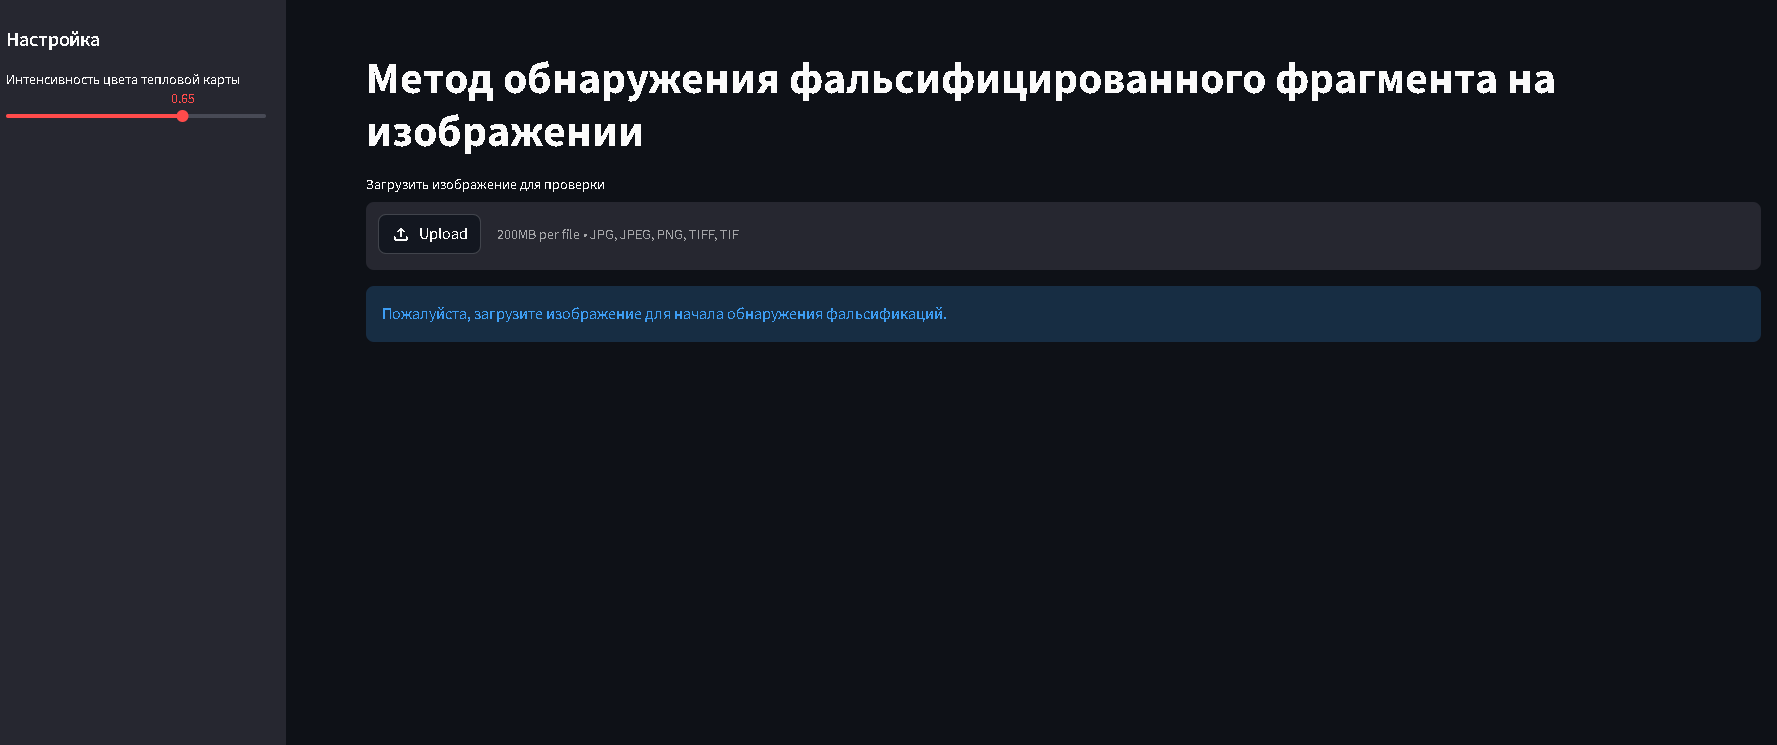
\includegraphics[,scale=0.35]{./img/3.1.png}
		\caption{Интерфейс пользователя.}  
		\label{img:interface}
\end{figure}

Интерфейс разделен на две основные части: панель настроек и область загрузки изображений. В разделе настроек пользователи могут настроить интенсивность цвета тепловой карты. Основная часть приложения сосредоточена на функции загрузки изображений, поддерживая перетаскивание файлов или ручной выбор в различных форматах для анализа и визуального отображения областей с искажениями в виде тепловых карт, бинарных масок.

После выбора пользователем файла изображения модель обработает его и выдаст результат. Если изображение не содержит фальсифицированного фрагмента, будет выдано сообщение, как показано на рисунке \ref{img:no_fake}.

\captionsetup{justification=centering,singlelinecheck=off}
\begin{figure}[h!]
	\centering
		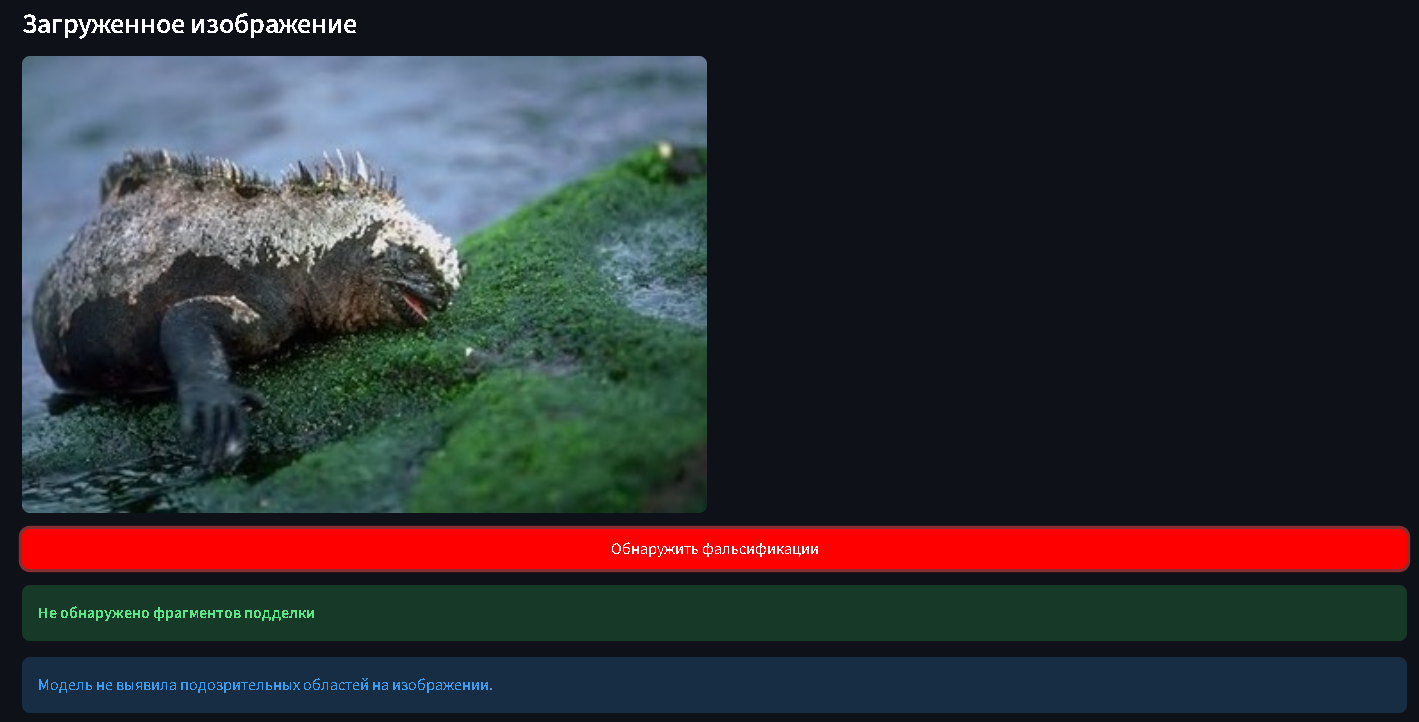
\includegraphics[,scale=0.45]{./img/3.2.png}
		\caption{Пример обнаружения при загрузке оригинального файла изображения}  
		\label{img:no_fake}
\end{figure}

Если загруженный файл изображения содержит фальсифицированные фрагменты, результатом будет изображение, содержащее ограничивающие рамки, указывающие области изображения, которые могут быть сфальсифицированы, процент сфальсифицированные пикселей и координаты этих ограничивающих рамок. Ниже, на рисунке \ref{img:fake}, приведён пример файла изображения, который иммет сфальсифицированные фрагменты.

\captionsetup{justification=centering,singlelinecheck=off}
\begin{figure}[h!]
	\centering
		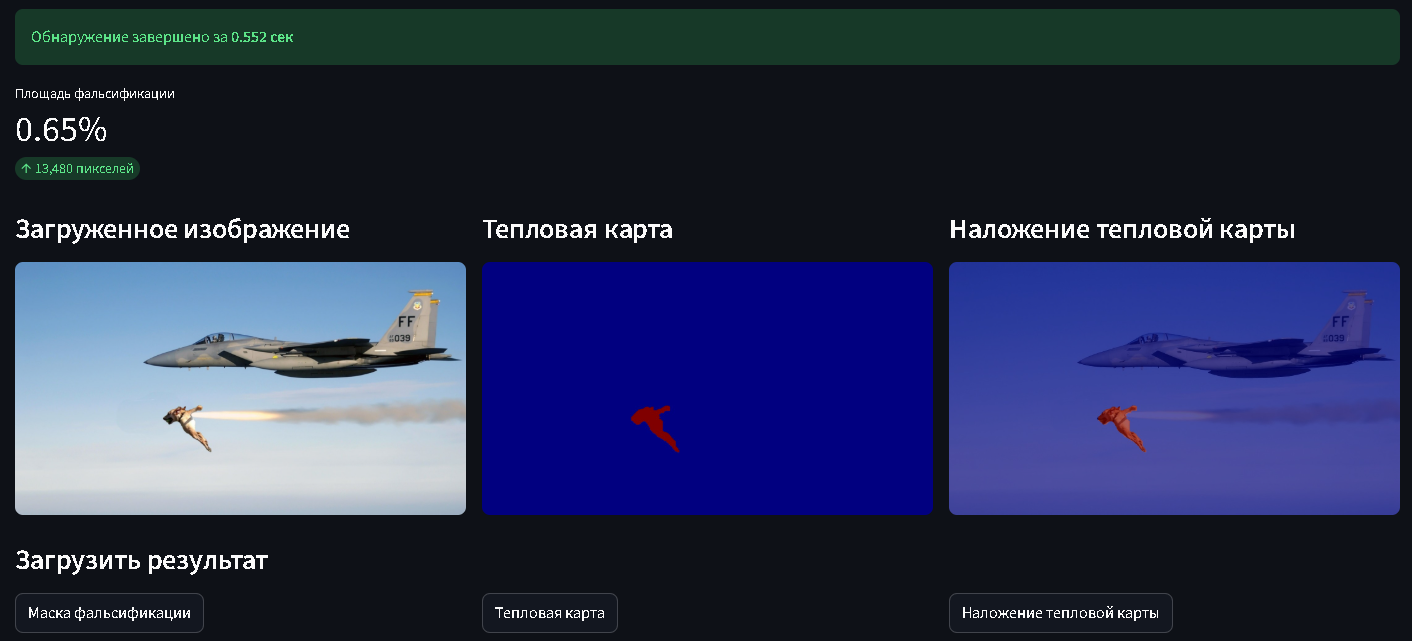
\includegraphics[,scale=0.45]{./img/3.3.png}
		\caption{Пример обнаружения при загрузке файла изображения, который содержит фальсифицированные фрагменты}  
		\label{img:fake}
\end{figure}
\newpage

\section*{Вывод}

В этом разделе были приведены выбор языка программирования и средства программирования и рассмотрены необходимые библиотеки, которые используются для разработки программного обеспечения. Также был описан формат входных и выходных данных. Также были приведены описание пользовательского интерфейса и руководство пользователя для установки и использования программного обеспечения.